\subsection*{Simulation: estimators perform better when their target matches the low-dimensional structure of the true covariance matrix}
\begin{figure}[htp]
\centering
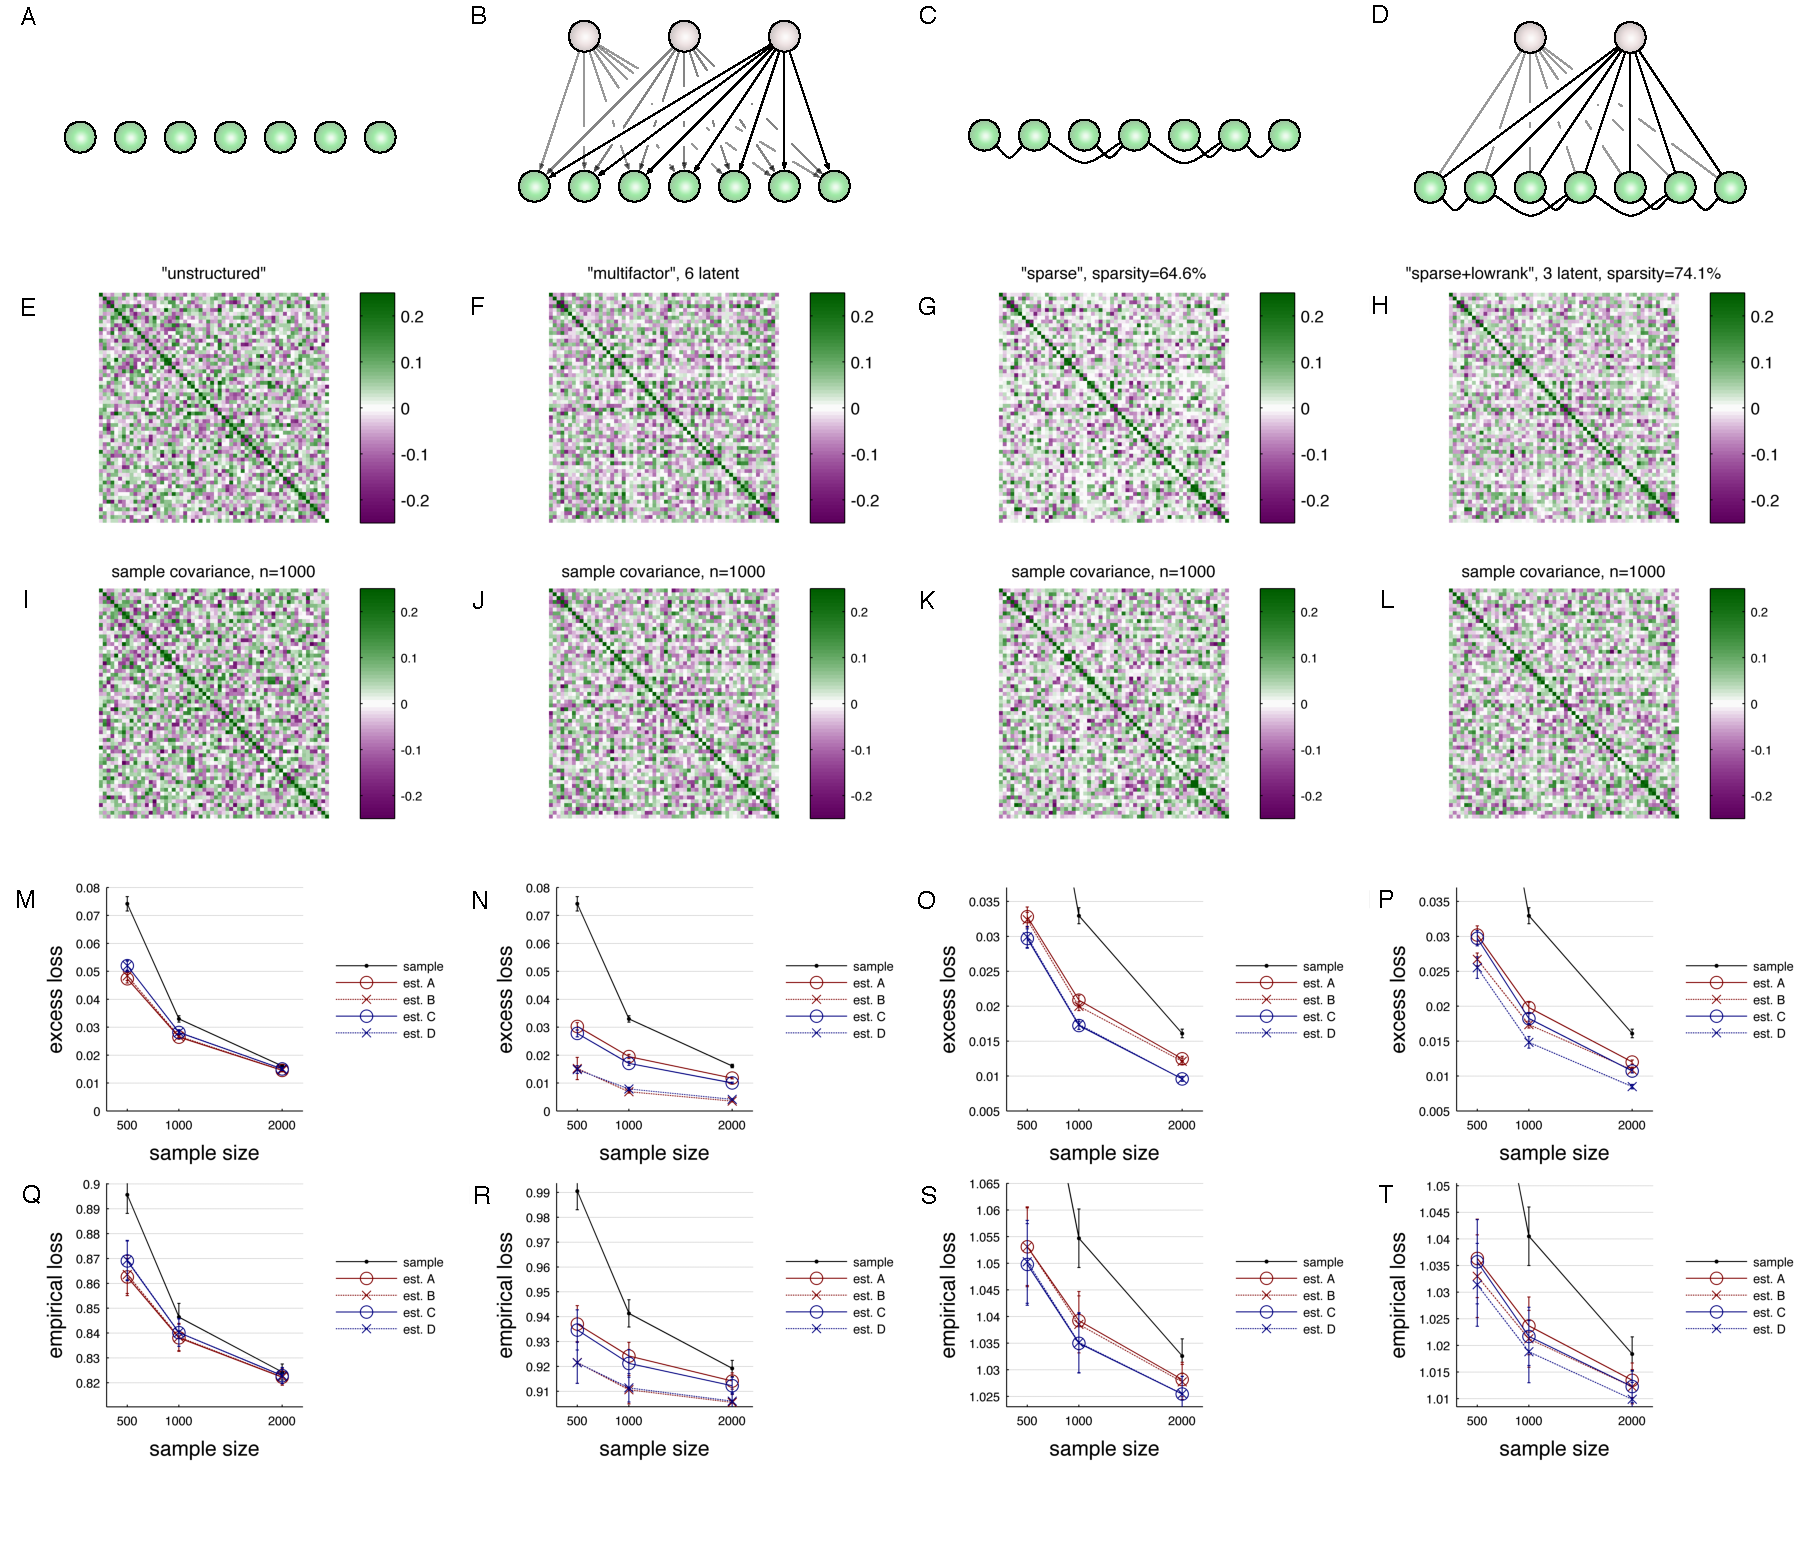
\includegraphics[width=1.0\textwidth]{figures/Figure3.pdf}
\caption{
Selection amongst estimators recognizes covariance atructure.
}\label{fig:03}
\end{figure}


Which covariance estimator is better is an empirical question.  The answer depends profoundly on the properties of the data generating system under investigation. 

A common misconception about regularization is that its effect depends on accurate prior knowlege about the structure of the data. However, substantial improvement can be attained by shrinking the unbiased estimate toward an arbitrary target as long as the target is less variable than the unbiased estimator.  This counter--intuitive phenomenon is known as \emph{Stein's phenomenon} or \emph{Stein's paradox} \cite{Efron:1977} named after its discoverer Charles Stein \cite{Stein:1956}.
The more accurate description of regularization is as of the optimal tradeoff between estimation and approximation error, the so-called ``bias-variance tradeoff'' as described in earlier sections. 
Taken in isolation, the fact that a given regularized estimator improves the estimate should not be interpreted to suggest that its target estimate has the same low-dimensional structure as the data generating process.   However, when multiple estimators are compared against each other, the ones whose target estimate can closely approximate the true value with the smallest number of parameters will be able to reduce the estimation error with mininimum increases in approximation error when compared against other estimators whose targets cannot consistenly approximate the true covariance matrix. 
\Kcomment{This seems a bit too wordy for the main part of the text.  I think the same can be said in a couple sentences.
People will likely wonder what this has to do with the analysis you are doing, if you spend too much time on generalities.} 

To illustrate the convergence of the four regularized covariance matrix estimators,  we constructed several kinds of covariance matrices to be used as the true covariance matrices for multivariate normal distributions to be used in simulations studies. Four of such true matrices, sized $100\times100$ are shown in Fig.~\ref{fig:03} A--D.  \Kcomment{What does the ``It'' in the following part of the text refer to?  Do you mean ``Each''?} It is computed as the sample covariance matrix of a finite sample (n=1000) drawn from a multivariate normal distribution with independent units and unit variances.  True matrix A has no low-dimensional structure: it takes $p\times(p+1)/2=5,050$ parameters to be fully defined.  True matrix B is computed by factor analysis from matrix A with $d=6$ factors.  As such, it has a low dimensional structure: it is fully defined with $p\times d +p = 700$ parameters.  True matrix C is computed by reducing to zero a large fraction the coefficients of the inverse of true matrix A \TODO{using GLASSO}. In this instance, 64.6\% of its off-diagonal elements are zero, and the entire matrix is fully defined with 1,825 parameters. Finally, true matrix D is an approximation of $A$ such that its inverse is a sum of a sparse matrix (74.1\% zeros of the digonal) and a low-rank component with rank $d=3$, with the number of parameters totaling 1582.

The true matrices B, C, and D correspond to Gaussian Graphical Models of the families depicted in Fig.~\ref{fig:02} B, C, and D, respectively. \TODO{Note that we do not have a true table that corresponds to the graphical model in Fig.~\ref{fig:02} simply because it is not of practical interest.}

Panels E, F, G, and H show sample covariance matrices computed from samples of 1000 independent observations from multivariate normal distributions with true covariance matrices in A, B, C, and D, respectively.  

Plots I, J, K, L show the quality of covariance matrix computed by the sample covariance matrix $\hat\Sigma_0$ as well as the four regularized covariance estimators $\mathcal A$, $\mathcal B$, $\mathcal C$, and $\mathcal D$.  Since we have access to the true covariance matrices, we use \emph{excess loss} $\loss{\hat\Sigma,\Sigma}-\loss{\Sigma,\Sigma}$ to evaluate the quality of the estimate $\hat\Sigma$. Excess loss approaches zero when the estimate coverges to the true value.  The error bars indicate the standard deviation (rather than standard error) for multiple samples drawn from the same true table.

All five covariance matrix estimators are \emph{consistent}: they converge to the true value as the sample size increases.   All regularized estimators dominate the sample covariance matrix independent of the low-dimensional structure of truth.  This is an example of Stein's phenomenon.  The regularized estimators are not equally \emph{efficient}: for a given sample size, some covariance estimators produce consistently lower loss than others.  Which estimator is most efficient depends on which estimator best matchest the low-dimensional structure of the true covariance matrix.  True covariance A does not have a low-dimensional structure and all four regularized estimators ($\mathcal A$,$\mathcal B$,$\mathcal C$,$\mathcal D$) perform similarly.  However, in cases when the true covariance matrix has a low-dimensional structure, the esimator whose target estimate can match that structure dominates the others.  Thus for truth B, estimator $\mathcal B$ domainates; for truth C, estimator $\mathcal C$ dominates; and for truth D,  estimator $\mathcal D$ dominates.  Note, however, that estimator $\mathcal D$'s target can accurately approximate the low dimensional structure of truths B and C and performed very closely to their matching estimators. \TODO{This does not mean however that we should design a ``universal'' estimator that can capture all kinds of low-dimensional structure because (a) it will fall for false patterns and (b) it will have a high number of hyperparameters, which will become intractable}.

Plots M, N, O, and P reproduce the same comparison as in I, J, K, and L but use validation loss from Eq.~\ref{eq:validationLoss} computed by 10-fold cross-validation.  This analysis is performed without access to the true covariance matrix and can thus be applied to empirical data.  The results are qualitatively comparable to those obtained with excess loss.  Because validation loss is computed by comparing estimates to noisy sample covariance matrices from smaller validation set, validation loss is a much noisier measurement than excess loss. In addition, validation loss converges to the unknown value $\loss{\Sigma,\Sigma}$ rather than zero.
